\documentclass[10pt,a4paper]{article}
\usepackage[utf8]{inputenc}
\usepackage{amsmath}
\usepackage{amsthm}
\usepackage{amsfonts}
\usepackage{amssymb}
\usepackage{multirow}
\usepackage{multicol}
\usepackage[spanish]{babel}
\usepackage{graphicx}
\usepackage[table]{xcolor}
\usepackage{wrapfig}
\usepackage{cite}
\usepackage{ieeetrantools}
\usepackage{float} 
\usepackage[margin=3.5cm]{geometry}
\hyphenation{Re-fe-ren-cias}
%\usepackage{color}              % For creating coloured text and background
\usepackage[hidelinks]{hyperref}            % For creating hyperlinks in cross references

\columnsep 0.8 cm
\pagestyle{empty}
\newtheorem{teorema}{Teorema}
\begin{document}
\renewcommand{\tablename}{Tabla}
\renewcommand{\refname}{Referencias bibliográficas.}
\bstctlcite{IEEEexample:BSTcontrol} % cambia "and" por "y" en bibliografa
\vspace{1cm}
\title{Sistema de Asistencia Basado en Reconocimiento Facial para la FPUNE}
\vspace{1cm}

\author{
    {\small Aldo Carrizo}\begin{scriptsize}$^{1}$\end{scriptsize},
    {\small Jorge Sanchez}\begin{scriptsize}$^{2}$\end{scriptsize}\\
    {\small Jorge Arrua}\begin{scriptsize}$^{2}$\end{scriptsize}\\
    {\small Facultad Politecnica, Universidad Nacional del Este}\\
    {\small Ciudad del Este - Paraguay}\\
    {\small aldocarrizo841@gmail.com}\begin{scriptsize}$^{1}$\end{scriptsize},
    {\small dani.sanchez.13.ds@gmail.com}\begin{scriptsize}$^{1}$\end{scriptsize},
    {\small jorgearrua@gmail.com}\begin{scriptsize}$^{2}$\end{scriptsize}
}
\date{}
\maketitle

\vspace*{-1cm}
%\begin{center} Fecha \end{center}

\begin{center}
\parbox{14 cm}{\abstract{
    
Este trabajo de investigación tiene como objetivo desarrollar un sistema automatizado de registro de asistencia basado en reconocimiento facial para la Facultad Politécnica de la Universidad Nacional del Este (FPUNE). Actualmente, el control de asistencia se realiza de forma manual, lo que genera errores y retrasa los procesos administrativos.

La solución propuesta emplea algoritmos de visión artificial e inteligencia artificial para detectar y reconocer rostros en tiempo real, automatizando el registro de asistencia. Se utilizaron herramientas como Python, OpenCV, TensorFlow y modelos como YOLOv8 y ArcFace. La metodología incluyó recolección de datos, entrenamiento de modelos y validación en un entorno real.

Los resultados muestran una alta precisión y eficiencia del sistema, incluso en condiciones variables. Además, se incorporó una plataforma para la justificación de ausencias por parte de los estudiantes. En conjunto, el sistema mejora la gestión académica, reduce errores humanos y optimiza el tiempo de los docentes.

\vspace*{0.1cm}
\noindent \textbf{Descriptores:} 1. Reconocimiento Facial, 2. Control de Asistencia, 3. Visión Artificial.

\begin{center}
\textbf{Abstract}
\end{center}

This research project aims to develop an automated attendance system based on facial recognition for the Polytechnic Faculty of the National University of the East (FPUNE). Currently, attendance is recorded manually, which often results in human errors and delays in administrative processes.

The proposed solution uses computer vision and artificial intelligence algorithms to detect and recognize faces in real time, automating the attendance process. Tools such as Python, OpenCV, TensorFlow, and models like YOLOv8 and ArcFace were used. The methodology included data collection, model training, and validation in a real environment.

The results demonstrate high accuracy and efficiency, even under variable conditions. The system also incorporates a platform that allows students to justify absences, streamlining validation by teachers. Overall, the solution enhances academic management by reducing manual workload and increasing transparency.

\vspace*{0.1cm}
\noindent \textbf{Key words:} 1. Facial Recognition, 2. Attendance Control, 3. Computer Vision.

}}
\end{center}
\vspace{.5cm}
\begin{multicols}{2}
\thispagestyle{empty}
\section{Introducción}

El registro de asistencia es una tarea clave en la gestión educativa y administrativa en instituciones académicas como la Facultad Politécnica de la Universidad Nacional del Este (FPUNE), desempeñando un rol fundamental en el seguimiento del desempeño estudiantil. Sin embargo, los métodos tradicionales de control manual mediante listas de asistencia suelen presentar errores humanos que afectan la precisión de los registros y la toma de decisiones académicas.

Este Trabajo Final de Grado (TFG) tiene como objetivo desarrollar un sistema automatizado basado en reconocimiento facial para optimizar el proceso de registro de asistencia en la FPUNE. Para ello, se utilizarán algoritmos avanzados de biometría facial que analizarán imágenes capturadas en tiempo real, asegurando así una identificación precisa y eficiente. Además, se ofrecerá una plataforma digital donde los estudiantes podrán justificar sus ausencias, y las autoridades correspondientes podrán gestionar estas justificaciones.

La metodología empleada comprende etapas de selección tecnológica, recopilación y procesamiento de imágenes, entrenamiento de modelos inteligentes y pruebas piloto en un entorno real durante un semestre académico del año 2025. Se espera que este sistema reduzca significativamente los errores actuales y mejore la gestión académica y administrativa, brindando datos más fiables y contribuyendo a una mayor eficiencia operativa.

Este estudio busca aportar información valiosa para estudiantes, docentes y autoridades, promoviendo una gestión académica más precisa y efectiva mediante la adopción de tecnologías innovadoras.
\subsection{Objetivos.}
\vspace{0.5cm}
\textit{Objetivo General}\\
Implementar un sistema de reconocimiento facial para el control de asistencia de estudiantes de la Facultad Politécnica de la Universidad Nacional del Este.

\vspace{0.5cm}
\textit{Objetivos Específicos}
\begin{enumerate}
    \item Seleccionar los algoritmos de reconocimiento facial.
    \item Seleccionar las herramientas tecnológicas para el desarrollo del Sistema.
    \item Identificar los requisitos para el desarrollo del sistema de registro de asistencia para la FPUNE.
    \item Desarrollar el sistema de reconocimiento facial y gestión de asistencias.
    \item Realizar pruebas de implementación.
    \item Evaluar resultados obtenidos.
\end{enumerate}

\subsection{Hipótesis}
El sistema de control de asistencia basado en reconocimiento facial registra
la asistencia de los estudiantes de la FPUNE.

\section{Discusión de literatura relevante.}
\subsection{Seguridad Biométrica}

Para abordar el concepto de seguridad biométrica, es fundamental primero comprender qué es la biometría. Es la ciencia del análisis de las características físicas o del comportamiento, propias de cada individuo, con el fin de autenticar su identidad. En el sentido literal y el más simple, la biometría significa la "medición del cuerpo humano"\cite{avastSeguridadBiometrica}.

La biometría es la medición estadística y matemática de características
físicas o biológicas únicas con fines de identificación\cite{thalesBiometria}.

Los datos biométricos son cualquier tipo de información sobre las características físicas de un individuo, como los patrones de la retina, las huellas dactilares y la estructura facial\cite{thalesBiometria}.

\begin{figure}[H]
  \centering
  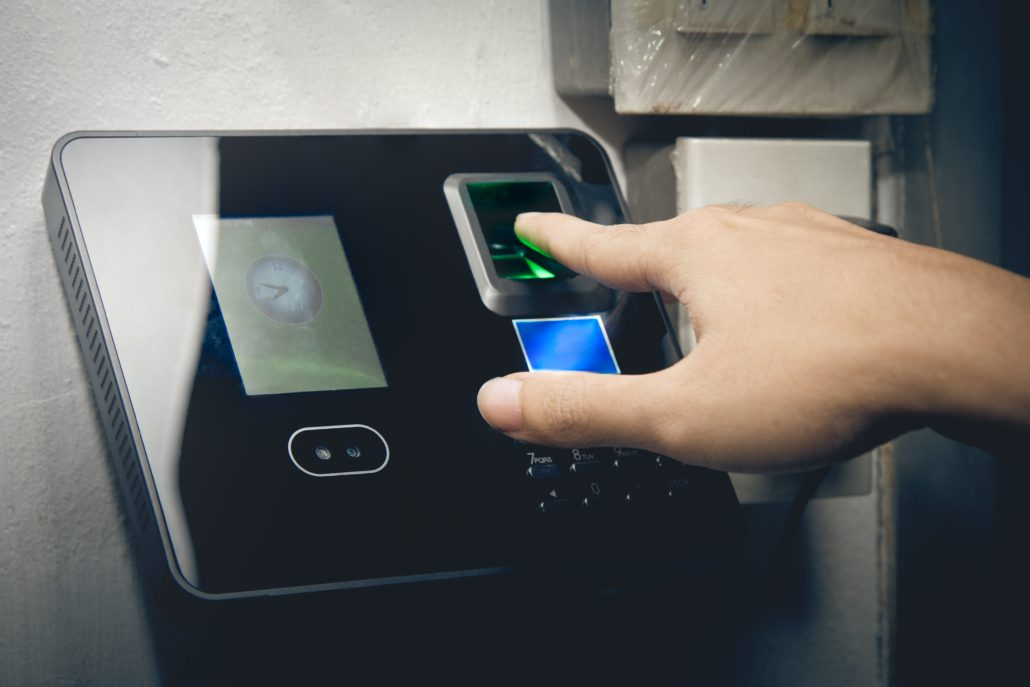
\includegraphics[width=0.4\textwidth]{imagenes_doc/segu_biometrica_1.jpg}
  \caption{Ejemplo de Seguridad Biométrica}\cite{beesafe_accesscontrol}.
  \label{fig:logo}
\end{figure}
\vspace{-0.5cm}

La seguridad biométrica se refiere al uso de características biológicas únicas para la autenticación digital y control de acceso. Los componentes de
hardware, como las cámaras o los lectores de huellas dactilares, recogen los
datos biométricos, que se escanean y se comparan algorítmicamente con la
información contenida en una base de datos. Si los dos conjuntos de datos
coinciden, se autentica la identidad y se concede el acceso\cite{thalesBiometria}.

\subsection{Reconocimiento Facial}

El reconocimiento facial es una manera de identificar o confirmar la identi
dad de una persona mediante su rostro. Los sistemas de reconocimiento facial
se pueden utilizar para identificar a las personas en fotos, videos o en tiempo
real\cite{reconocimientoKaspersky}.

\begin{figure}[H]
  \centering
  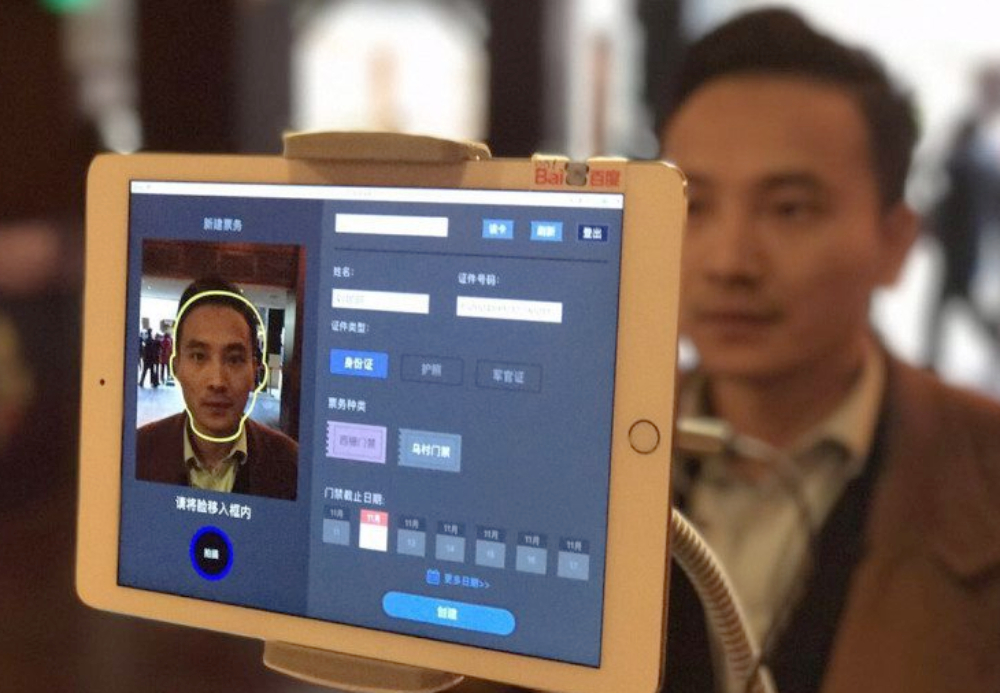
\includegraphics[width=0.4\textwidth]{imagenes_doc/Reconocimiento_Facial.jpg}
  \caption{Dispositivo de reconocimiento facial utilizado en un aeropuerto para verificar la identidad de los pasajeros mediante el análisis de sus rasgos faciales en tiempo real\cite{aeropuertosJapon}.}
  \label{fig:logo}
\end{figure}

El reconocimiento facial es una categoría de seguridad biométrica. Otras
formas de software biométrico incluyen el reconocimiento de voz, el reconoci
miento de huellas digitales y el reconocimiento de retina o iris. La tecnología
se utiliza principalmente para la protección y las fuerzas de seguridad, aunque
hay un creciente interés en otras áreas de uso\cite{reconocimientoKaspersky}.

\subsection{Inteligencia Artificial}
La inteligencia artificial es un campo de la ciencia relacionado con la creación de computadoras y máquinas que pueden razonar, aprender y actuar de una manera que normalmente requeriría inteligencia humana o que involucra datos cuya escala excede lo que los humanos pueden analizar.

La IA es un campo amplio que incluye muchas disciplinas, como la informática, el análisis y la estadística de datos, la ingeniería de hardware y software, la lingüística, la neurociencia y hasta la filosofía y la psicología.

La inteligencia artificial es un conjunto de tecnologías que se basan principalmente en el aprendizaje automático y el aprendizaje profundo, que se usan para el análisis de datos, la generación de predicciones y previsiones, la categorización de objetos, el procesamiento de lenguaje natural, las recomendaciones, la recuperación inteligente de datos y mucho más \cite{aiIBM}.

\subsection{Registros Académicos.}
Los registros académicos son la recopilación sistemática de información relacionada con el desempeño, progreso y trayectoria académica de un estudiante. Esta información se almacena en diversos formatos (digitales o físicos) y es administrada por instituciones educativas, como escuelas, colegios, universidades, etc\cite{registroAsistenciaUTA}.
\begin{figure}[H]
  \centering
  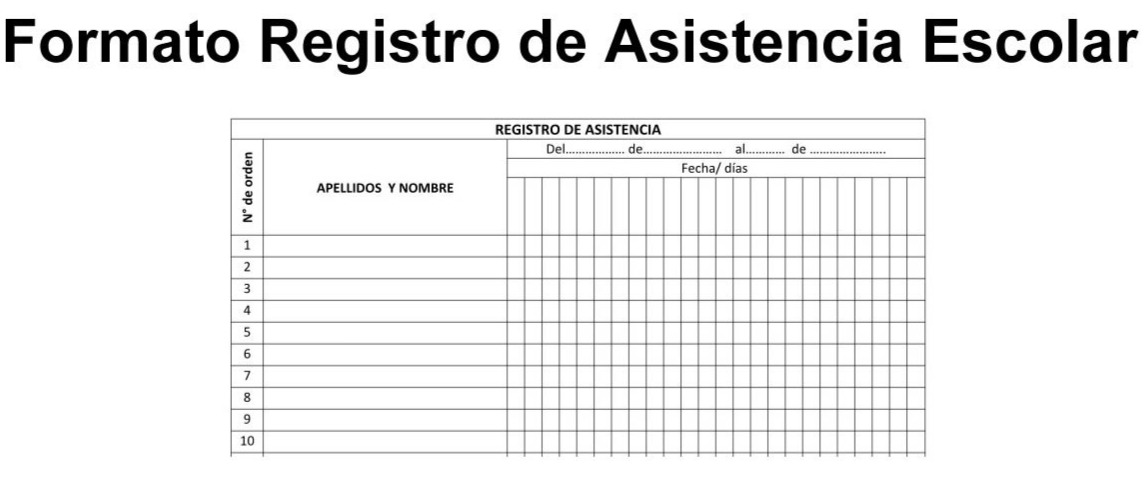
\includegraphics[width=0.5\textwidth]{imagenes_doc/registroimg.jpg}
  \caption{La imagen muestra un formato tradicional de registro de asistencia escolar, utilizado por docentes para anotar la presencia diaria de los alumnos a lo largo de un período determinado\cite{listaAsistenciaEscolar}.}
  \label{fig:logo}
\end{figure}
\vspace{-1cm}

\section{Método.}
Este trabajo se enmarca dentro de una investigación aplicada tecnológica orientada al diseño e implementación de un sistema automatizado para el control de asistencia, utilizando técnicas de reconocimiento facial. A continuación, se detallan las fases metodológicas y técnicas del proyecto, desde la planificación inicial hasta las pruebas en un entorno académico real.

El enfoque adoptado combina elementos de investigación cualitativa y cuantitativa. Por un lado, se recogen percepciones y experiencias de los usuarios mediante entrevistas, y por otro, se analizan métricas de rendimiento del sistema como precisión y velocidad de procesamiento.\\

\textbf{\textit{Enfoque metodológico}}\\
El enfoque metodológico del proyecto es mixto. Se recurrió al análisis cuantitativo para evaluar el desempeño del sistema (precisión de reconocimiento, cantidad de asistencias correctamente registradas, etc.), y al análisis cualitativo para conocer las opiniones y experiencias de los usuarios (docentes y estudiantes).

Se trata de una investigación descriptiva, no experimental y longitudinal. El sistema fue implementado en un entorno académico real durante un semestre en la FPUNE, lo cual permitió observar su funcionamiento a lo largo del tiempo y realizar ajustes progresivos.


\subsection{Instrumentos}

Para el desarrollo del sistema se utilizaron diversas herramientas tecnológicas, seleccionadas por su utilidad y eficiencia en proyectos de desarrollo de software con componentes de visión artificial.

Se empleó \textbf{Figma} para el diseño de la interfaz de usuario, \textbf{Visual Studio Code} como entorno principal de codificación, y \textbf{Git} junto con \textbf{GitHub Desktop} para el control de versiones. El sistema fue programado en \textbf{Python}, utilizando \textbf{YOLO} para la detección de rostros y \textbf{ArcFace} para el reconocimiento facial. Los datos fueron almacenados y gestionados mediante \textbf{PostgreSQL} utilizando \textbf{SQL} como lenguaje de consulta.

Estas herramientas permitieron una integración eficaz de los componentes del sistema, garantizando un desarrollo ágil y una correcta implementación del modelo en tiempo real.


\section{Resultados.}

Durante la etapa de pruebas, se identificaron ciertos errores recurrentes en el funcionamiento del sistema, principalmente relacionados con la precisión del reconocimiento facial. A continuación, se presenta una tabla con los tipos de errores detectados, su causa y las acciones de mitigación implementadas para mejorar el desempeño.

\begin{table}[H]
    \centering
    \caption{Errores frecuentes y acciones de mitigación}
    \label{tab:errores_ajustes}
    \renewcommand{\arraystretch}{1.3}
    \begin{tabular}{|p{2cm}|p{2cm}|p{2cm}|}
        \hline
        \textbf{Tipo de error} & \textbf{Causa identificada} & \textbf{Ajuste o solución aplicada} \\
        \hline
        Falsos positivos en la identificación facial & Umbral de similitud fijo (50) no adecuado para la variabilidad de datos por usuario & Se ajustó el umbral dinámicamente según la cantidad de imágenes por usuario y su variación interna \\
        \hline
        Reconocimiento erróneo con poca iluminación & Capturas de imágenes en condiciones de baja luz o sombras parciales & Se incorporó preprocesamiento de imagen (mejora de contraste y normalización) \\
		\hline
		Procesamiento lento con gran volumen de usuarios & Comparación secuencial con todos los embeddings registrados & Se implementó filtrado previo por clase probable y limitación del número de comparaciones activas \\
		\hline
    \end{tabular}
\end{table}
\vspace{-1cm}

\begin{table}[H]
\centering
\caption{Configuración de umbral vs. resultado esperado}
\label{tab:umbral_similitud}
\renewcommand{\arraystretch}{1.3}
\scriptsize
\begin{tabular}{|p{1cm}|p{0.9cm}|p{1.8cm}|p{1.5cm}|}
\hline
\hline
$> 1.8$ & $100 - \texttt{dist} \times 20$ & Reconoce con más flexibilidad & Acepta diferencias de expresión o iluminación \\
\hline
$> 3.5$ & $100 - \texttt{dist} \times 18$ & Tolerante, puede haber falsos positivos & Útil si los embeddings fueron generados con solo 1 o 2 imágenes \\
\hline
$> 5.0$ & $100 - \texttt{dist} \times 15$ & Muy laxo, reconoce casi todo & Solo útil para pruebas \\
\hline
\end{tabular}
\end{table}
\vspace{-1cm}


\textbf{Configuración 1: Umbral 1.8 y factor 20}

\begin{figure}[H]
    \centering
    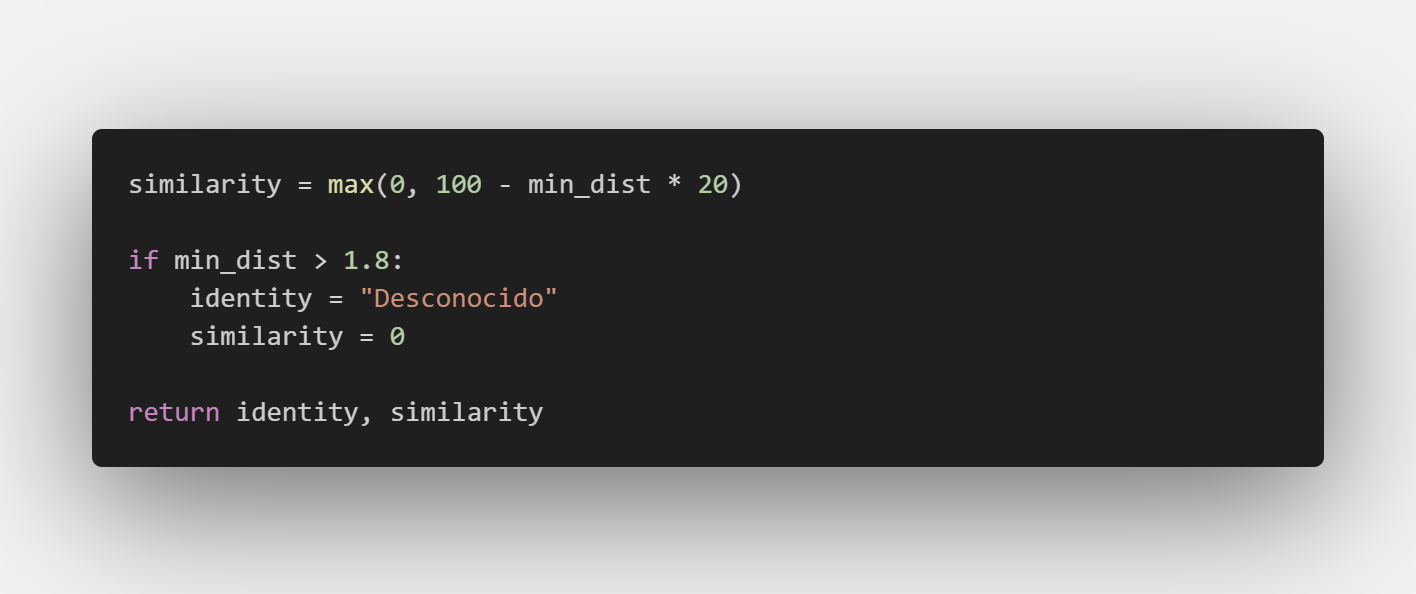
\includegraphics[width=0.4\textwidth]{imagenes/3.png}
    \caption{Fragmento de código utilizado para configurar el umbral de reconocimiento facial.}
\end{figure}
\vspace{-0.5cm}

\begin{figure}[H]
    \centering
    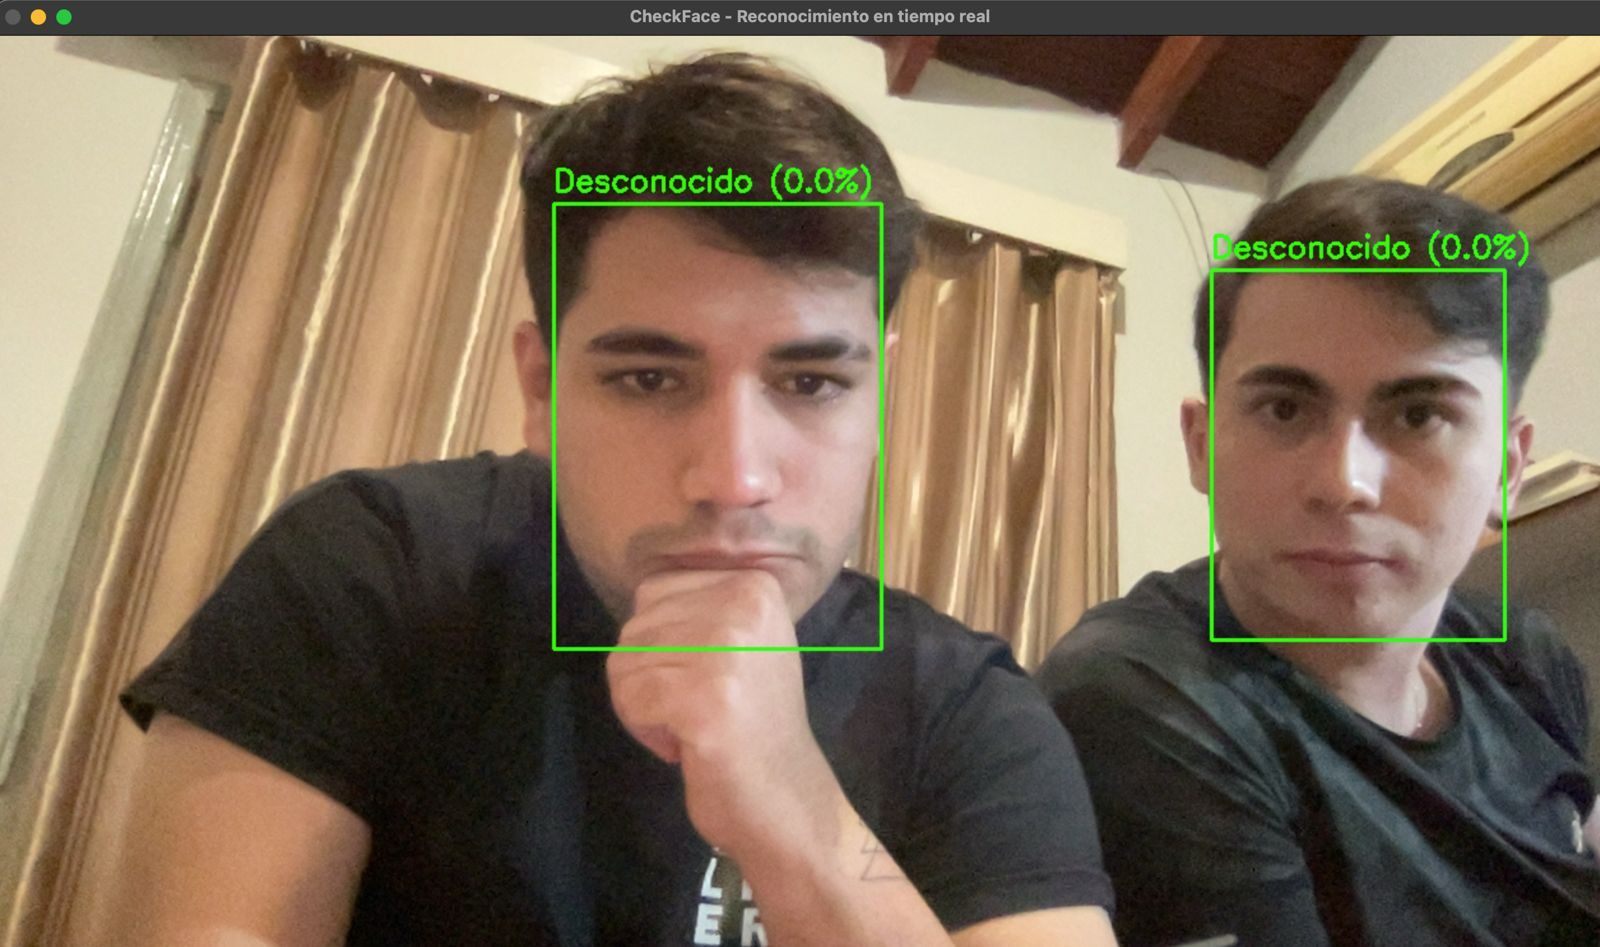
\includegraphics[width=0.4\textwidth]{imagenes/umbral1.8min_dist20.jpg}
    \caption{Resultados obtenidos aplicando la configuración anterior (umbral = 1.8 y factor de similitud 20).}
\end{figure}


\textbf{Configuración 2: Umbral 3.5 y factor 18}

\begin{figure}[H]
    \centering
    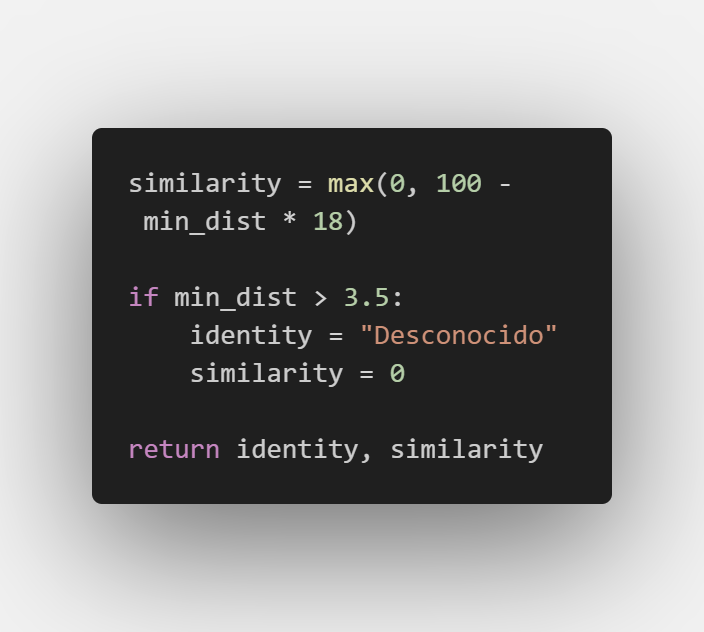
\includegraphics[width=0.4\textwidth]{imagenes/4.png}
    \caption{Fragmento de código utilizado para configurar el umbral de reconocimiento facial.}
\end{figure}
\vspace{-0.5cm}

\begin{figure}[H]
    \centering
    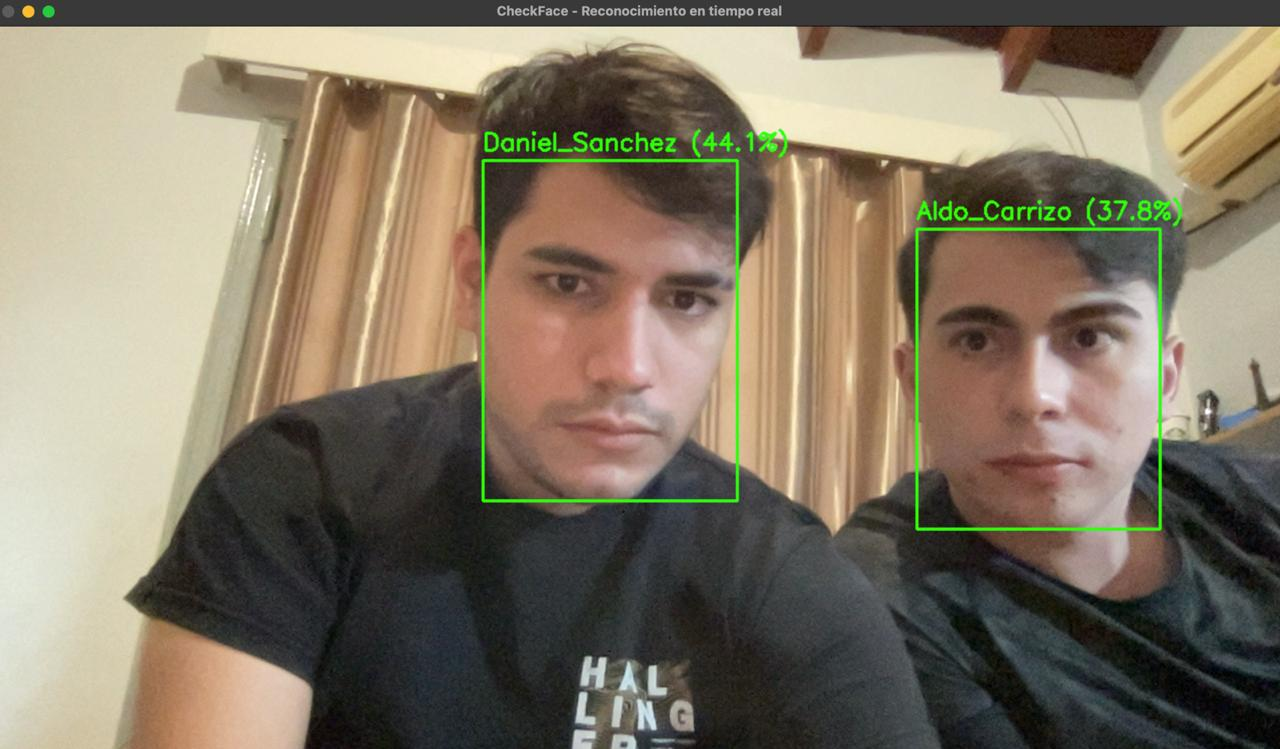
\includegraphics[width=0.4\textwidth]{imagenes/4.4.jpg}
    \caption{Resultados obtenidos aplicando la configuración anterior (umbral = 3.5 y factor de similitud 18).}
\end{figure}




\textbf{Configuración 3: Umbral 5 y factor 15}

\begin{figure}[H]
    \centering
    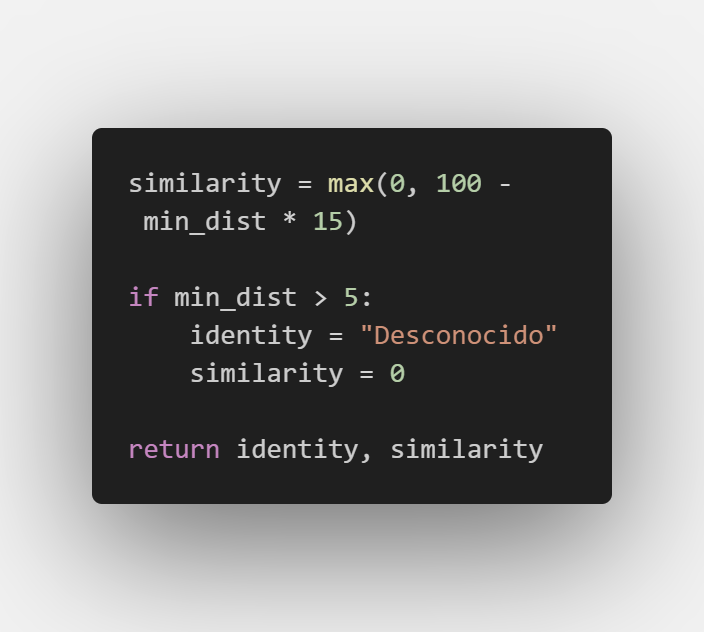
\includegraphics[width=0.4\textwidth]{imagenes/5.png}
    \caption{Fragmento de código utilizado para configurar el umbral de reconocimiento facial.}
\end{figure}
\vspace{-0.5cm}

\begin{figure}[H]
    \centering
    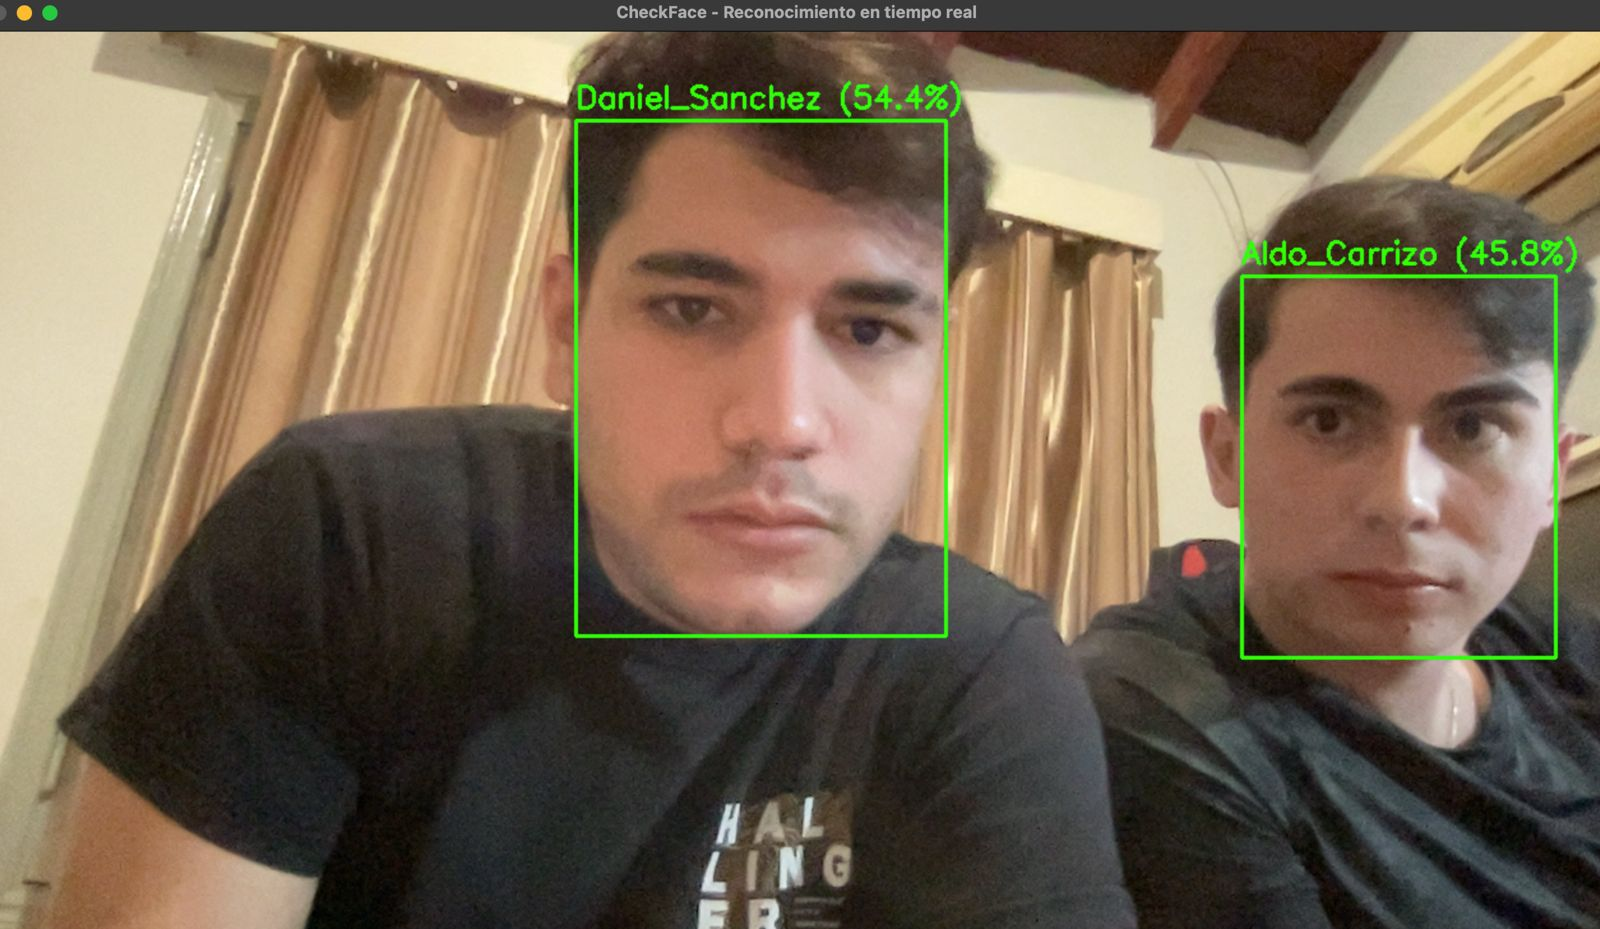
\includegraphics[width=0.4\textwidth]{imagenes/5.5.jpg}
    \caption{Resultados obtenidos aplicando la configuración anterior (umbral = 5 y factor de similitud 15).}
\end{figure}



\section{Discusión.}

El desarrollo del sistema automatizado de control de asistencia mediante reconocimiento facial en la FPUNE permitió abordar una problemática concreta y recurrente: la necesidad de una gestión precisa, ágil y confiable de la asistencia estudiantil. La investigación cumplió con los objetivos propuestos y logró una solución funcional basada en tecnologías de visión artificial.

Los resultados experimentales mostraron que, al configurar adecuadamente parámetros como el umbral de similitud (entre 1.0 y 1.8), se alcanzó un desempeño óptimo en términos de precisión y velocidad, reduciendo eficazmente los falsos positivos. Esto refuerza la aplicabilidad del sistema en entornos reales y coincide con hallazgos previos sobre la sensibilidad de los sistemas biométricos ante variaciones de iluminación, ángulo y calidad de imagen.

Modelos como YOLOv8n-Face y ArcFace demostraron ser opciones viables por su buen equilibrio entre precisión, rendimiento y tamaño, especialmente útiles en contextos con recursos limitados. No obstante, se identificaron limitaciones relacionadas con las condiciones de captura y la necesidad de múltiples imágenes por usuario.

La implementación evidenció que la automatización del control de asistencia es viable técnica y administrativamente, reduciendo errores humanos y optimizando procesos. En consecuencia, el sistema desarrollado representa una solución concreta con potencial de adopción institucional.


\bibliographystyle{IEEEtran-castellano}

\bibliography{test}

\end{multicols}

\end{document}